\documentclass{beamer}\usepackage[]{graphicx}\usepackage[]{color}
%% maxwidth is the original width if it is less than linewidth
%% otherwise use linewidth (to make sure the graphics do not exceed the margin)
\makeatletter
\def\maxwidth{ %
  \ifdim\Gin@nat@width>\linewidth
    \linewidth
  \else
    \Gin@nat@width
  \fi
}
\makeatother

\definecolor{fgcolor}{rgb}{0.196, 0.196, 0.196}
\newcommand{\hlnum}[1]{\textcolor[rgb]{0.063,0.58,0.627}{#1}}%
\newcommand{\hlstr}[1]{\textcolor[rgb]{0.063,0.58,0.627}{#1}}%
\newcommand{\hlcom}[1]{\textcolor[rgb]{0.588,0.588,0.588}{#1}}%
\newcommand{\hlopt}[1]{\textcolor[rgb]{0.196,0.196,0.196}{#1}}%
\newcommand{\hlstd}[1]{\textcolor[rgb]{0.196,0.196,0.196}{#1}}%
\newcommand{\hlkwa}[1]{\textcolor[rgb]{0.231,0.416,0.784}{#1}}%
\newcommand{\hlkwb}[1]{\textcolor[rgb]{0.627,0,0.314}{#1}}%
\newcommand{\hlkwc}[1]{\textcolor[rgb]{0,0.631,0.314}{#1}}%
\newcommand{\hlkwd}[1]{\textcolor[rgb]{0.78,0.227,0.412}{#1}}%
\let\hlipl\hlkwb

\usepackage{framed}
\makeatletter
\newenvironment{kframe}{%
 \def\at@end@of@kframe{}%
 \ifinner\ifhmode%
  \def\at@end@of@kframe{\end{minipage}}%
  \begin{minipage}{\columnwidth}%
 \fi\fi%
 \def\FrameCommand##1{\hskip\@totalleftmargin \hskip-\fboxsep
 \colorbox{shadecolor}{##1}\hskip-\fboxsep
     % There is no \\@totalrightmargin, so:
     \hskip-\linewidth \hskip-\@totalleftmargin \hskip\columnwidth}%
 \MakeFramed {\advance\hsize-\width
   \@totalleftmargin\z@ \linewidth\hsize
   \@setminipage}}%
 {\par\unskip\endMakeFramed%
 \at@end@of@kframe}
\makeatother

\definecolor{shadecolor}{rgb}{.97, .97, .97}
\definecolor{messagecolor}{rgb}{0, 0, 0}
\definecolor{warningcolor}{rgb}{1, 0, 1}
\definecolor{errorcolor}{rgb}{1, 0, 0}
\newenvironment{knitrout}{}{} % an empty environment to be redefined in TeX

\usepackage{alltt}

% load packages
\usepackage{tikz}
\usepackage{graphicx}
\usepackage{upquote}
\usepackage{listings}
\usepackage{hyperref}
\usepackage{color}
\usepackage{lmodern}



% define a bunch of colors
\definecolor{gray}{RGB}{110,110,110}
\definecolor{darkgray}{RGB}{100,100,100}
\definecolor{lightgray}{RGB}{200,200,200}
\definecolor{lightgrey}{RGB}{200,200,200}
\definecolor{turquoise}{RGB}{81,193,188}
\definecolor{mamey}{RGB}{255,107,107}
\definecolor{tomato}{RGB}{255,136,136}
\definecolor{mandarina}{RGB}{229,169,25}
\definecolor{lemon}{rgb}{0.81,0.95,0.29}
\definecolor{bluesky}{rgb}{0.71,0.81,0.96}
\definecolor{chiclamino}{RGB}{107,174,214}
\definecolor{violet}{RGB}{133,135,211}

\definecolor{foreground}{RGB}{81,141,193}
\definecolor{background}{RGB}{246,244,240}
\definecolor{highlight}{RGB}{229,169,25}
\definecolor{lowlight}{RGB}{200,200,200}

% setting beamer colors
\setbeamercolor{title}{fg=lightgray}
\setbeamercolor{frametitle}{fg=lightgray}
\setbeamercolor{block title}{fg=turquoise}
\setbeamercolor{structure}{fg=turquoise}
\setbeamercolor{titlelike}{fg=title}
\setbeamercolor{subtitle}{fg=turquoise}
\setbeamercolor{institute}{fg=gray}
\setbeamercolor{normal text}{fg=gray,bg=background}

\setbeamercolor{palette primary}{fg=lightgray}
\setbeamercolor{palette secondary}{fg=lightgray}
\setbeamercolor{palette tertiary}{fg=lightgray}

\setbeamerfont{itemize/enumerate subbody}{size=\footnotesize}
\setbeamerfont{itemize/enumerate subitem}{size=\footnotesize}

\hypersetup{
  colorlinks=true,
  urlcolor=tomato,
  linkcolor=lightgray
}

% commands
\newcommand{\code}[1]{\texttt{#1}}
\newcommand{\high}[1]{\textcolor{highlight}{#1}}
\newcommand{\low}[1]{\textcolor{lowlight}{#1}}
\newcommand{\highcode}[1]{\textcolor{highlight}{\texttt{#1}}}


%\usecolortheme{rose}
\setbeamertemplate{blocks}[rounded]
\setbeamertemplate{footline}[frame number] 
\setbeamertemplate{navigation symbols}{}
\setbeamertemplate{frametitle}[default][center]
\useoutertheme{infolines}  % add footlines
\setbeamersize{text margin left=25pt,text margin right=25pt}



% to remove empty brackets of \institution
\makeatletter
\setbeamertemplate{footline}
{
  \leavevmode%
  \hbox{%
  \begin{beamercolorbox}[wd=.333333\paperwidth,ht=2.25ex,dp=1ex,center]{author in head/foot}%
    \usebeamerfont{author in head/foot}\insertshortauthor%~~\beamer@ifempty{\insertshortinstitute}{}{(\insertshortinstitute)}
  \end{beamercolorbox}%
  \begin{beamercolorbox}[wd=.333333\paperwidth,ht=2.25ex,dp=1ex,center]{title in head/foot}%
    \usebeamerfont{title in head/foot}\insertshorttitle
  \end{beamercolorbox}%
  \begin{beamercolorbox}[wd=.333333\paperwidth,ht=2.25ex,dp=1ex,right]{date in head/foot}%
    \usebeamerfont{date in head/foot}\insertshortdate{}\hspace*{2em}
    \insertframenumber{} / \inserttotalframenumber\hspace*{2ex} 
  \end{beamercolorbox}}%
  \vskip0pt%
}
\makeatother



\title[Getting data from the web with R]{\LARGE Getting Data from the Web with R} 
\subtitle[Web Data in R]{\large Part 2: Reading Files from the Web}
\author[gastonsanchez.com]{
 \textcolor{gray}{\textbf{G}aston \textbf{S}anchez}
}
\institute[]{\scriptsize \textcolor{lightgray}{April-May 2014}}
\date[CC BY-SA-NC 4.0]{
 \textcolor{lightgray}{\tiny{Content licensed under 
 \href{http://creativecommons.org/licenses/by-nc-sa/4.0/}{CC BY-NC-SA 4.0}}}
}
\IfFileExists{upquote.sty}{\usepackage{upquote}}{}
\begin{document}




%--- the titlepage frame -------------------------%

\begin{frame}[plain]
 \titlepage
\end{frame}

%------------------------------------------------

{ % all template changes are local to this group.
    \setbeamertemplate{navigation symbols}{}
    \begin{frame}[plain]
        \begin{tikzpicture}[remember picture,overlay]
            \node[at=(current page.center)] {
                
\includegraphics[width=\paperwidth]{images/web2r.pdf}
            };
        \end{tikzpicture}
     \end{frame}
}

%------------------------------------------------

\begin{frame}[fragile]
\frametitle{Readme}

\begin{block}{\scriptsize License:}
\tiny
 \begin{itemize}
  \item[] Creative Commons Attribution-NonCommercial-ShareAlike 4.0 International License \\ 
  \url{http://creativecommons.org/licenses/by-nc-sa/4.0/}{}
 \end{itemize}
\end{block}

\begin{block}{\scriptsize You are free to:}
\tiny
 \begin{itemize}
  \item[] \textcolor{darkgray}{\textbf{Share}} --- \textcolor{gray}{copy and redistribute the material}
  \item[] \textcolor{darkgray}{\textbf{Adapt}} --- \textcolor{gray}{rebuild and transform the material}
 \end{itemize}
\end{block}

\vspace{2mm}
\begin{block}{\scriptsize Under the following conditions:}
\tiny
\begin{itemize}
 \item[] \textcolor{darkgray}{\textbf{Attribution}} --- \textcolor{gray}{You must give appropriate credit, provide a link to the license, and indicate if changes were made.}
 \item[] \textcolor{darkgray}{\textbf{NonCommercial}} --- \textcolor{gray}{You may not use this work for commercial purposes.}
 \item[] \textcolor{darkgray}{\textbf{Share Alike}} --- \textcolor{gray}{If you remix, transform, or build upon this 
 work, you must distribute your contributions under the same license to this one.}
\end{itemize}
\end{block}

\end{frame}

%------------------------------------------------

\begin{frame}
\frametitle{Lectures Menu}

\begin{columns}[t]
\begin{column}{0.1\textwidth}
%--- empty space ---%
\end{column}
\begin{column}{0.8\textwidth}
 \begin{block}{Slide Decks}
  \begin{enumerate}
   \item \textcolor{lightgray}{Introduction}
   \item \textbf{Reading files from the Web}
   \item \textcolor{lightgray}{Basics of XML and HTML}
   \item \textcolor{lightgray}{Parsing XML / HTML content}
   \item \textcolor{lightgray}{Handling JSON data}
   \item \textcolor{lightgray}{HTTP Basics and the RCurl Package}
   \item \textcolor{lightgray}{Getting data via Web Forms}
   \item \textcolor{lightgray}{Getting data via Web APIs}
  \end{enumerate}
 \end{block}
\end{column}
\begin{column}{0.1\textwidth}
%--- empty space ---%
\end{column}
\end{columns}

\end{frame}

%------------------------------------------------

\begin{frame}
 \begin{center}
  \Huge{\textcolor{mandarina}{Reading Files \\ from the Web}}
 \end{center}
\end{frame}

%------------------------------------------------

\begin{frame}
\frametitle{Data Files from the Web...}

\begin{columns}[t]
\begin{column}{0.5\textwidth}
 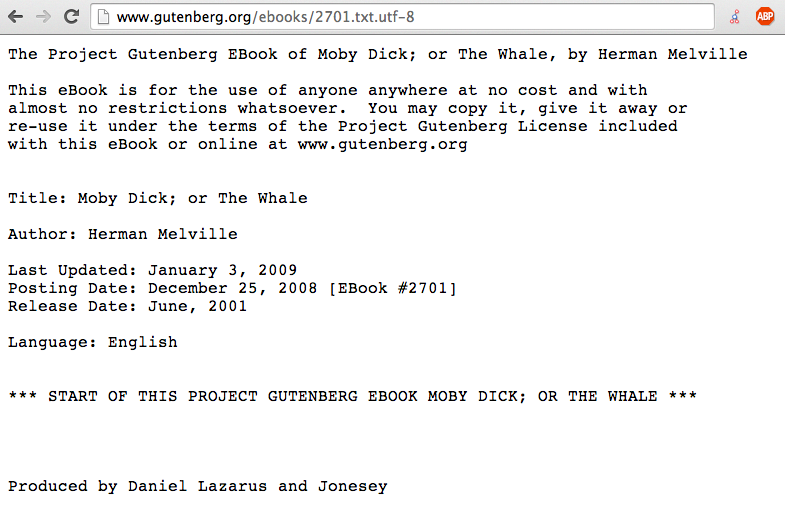
\includegraphics[width=4.5cm]{images/moby_dick_book.png}
\end{column}
\begin{column}{0.5\textwidth}
 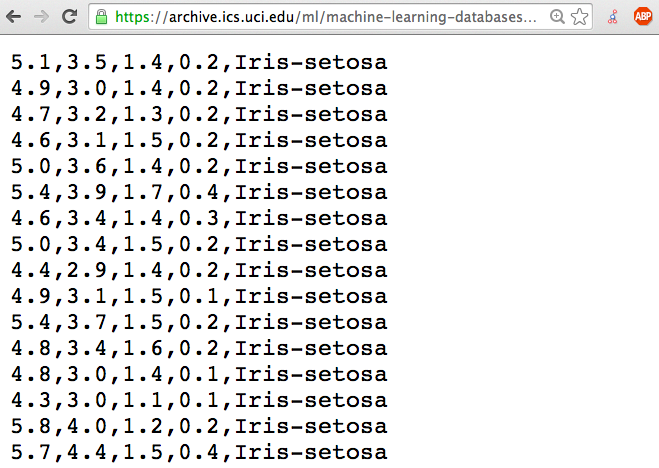
\includegraphics[width=4.5cm]{images/iris_data.png}
\end{column}
\end{columns}

\vspace{5mm}

\begin{columns}[t]
\begin{column}{0.5\textwidth}
 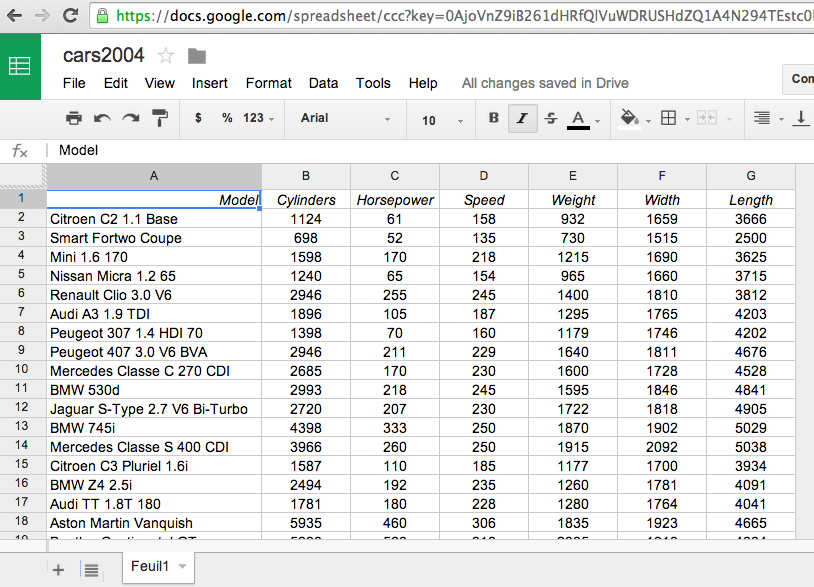
\includegraphics[width=4.5cm]{images/cars2004_data.png}
\end{column}
\begin{column}{0.5\textwidth}
 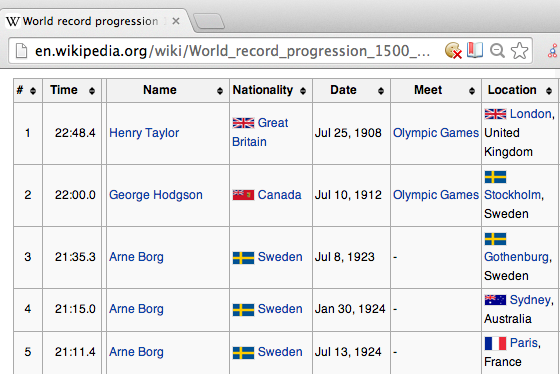
\includegraphics[width=4.5cm]{images/wikipedia_table.png}
\end{column}
\end{columns}

\end{frame}

%------------------------------------------------

\begin{frame}
\frametitle{Goal}

\begin{columns}[t]
\begin{column}{0.1\textwidth}
%--- empty space ---%
\end{column}
\begin{column}{0.8\textwidth}

\begin{block}{From the web to R}
The goal of these slides is to show you \textbf{different ways to read (data) files from the Web} into R
\end{block}

\end{column}
\begin{column}{0.1\textwidth}
%--- empty space ---%
\end{column}
\end{columns}

\end{frame}

%------------------------------------------------

\begin{frame}
\frametitle{Synopsis}

\begin{columns}[t]
\begin{column}{0.1\textwidth}
%--- empty space ---%
\end{column}
\begin{column}{0.8\textwidth}

\begin{block}{In a nutshell}
We'll cover a variety of situations you most likely will find yourself dealing with:
\begin{itemize}
 \item reading raw (plain) text
 \item reading tabular (spreadsheet-like) data
 \item reading structured data (xml, html) as text
 \item reading R scripts and Rdata files
\end{itemize}
\end{block}

\end{column}
\begin{column}{0.1\textwidth}
%--- empty space ---%
\end{column}
\end{columns}

\end{frame}

%------------------------------------------------

\begin{frame}
\frametitle{Some References}

\begin{itemize}
 \item R Data Import / Export Manual \\
 \low{by R Core Team}
 \item Data Manipulation with R \\
 \low{by Phil Spector}
 \item R Programming for Bioinformatics \\
 \low{by Robert Gentleman}
 \item The Art of R Programming \\
 \low{by Norm Matloff}
 \item XML and Web Technlogies for Data Sciences with R \\
 \low{by Deb Nolan and Duncan Temple Lang}
\end{itemize}

\end{frame}

%------------------------------------------------

\begin{frame}
\frametitle{Considerations}

\begin{columns}[t]
\begin{column}{0.1\textwidth}
%--- empty space ---%
\end{column}
\begin{column}{0.8\textwidth}

\begin{block}{Keep in mind}
All the material described in this presentation relies on 3 key assumptions:  
\begin{itemize}
 \item we know \high{where} the data is located
 \item we know \high{how} the data is stored (i.e. type of file)
 \item all we want is to import the data in R
\end{itemize}
\end{block}

\end{column}
\begin{column}{0.1\textwidth}
%--- empty space ---%
\end{column}
\end{columns}

\end{frame}

%------------------------------------------------

\begin{frame}
 \begin{center}
  \Huge{\textcolor{mandarina}{Reading Files \\ from the Web}}
 \end{center}
\end{frame}

%------------------------------------------------

{ % all template changes are local to this group.
    \setbeamertemplate{navigation symbols}{}
    \begin{frame}[plain]
        \begin{tikzpicture}[remember picture,overlay]
            \node[at=(current page.center)] {
                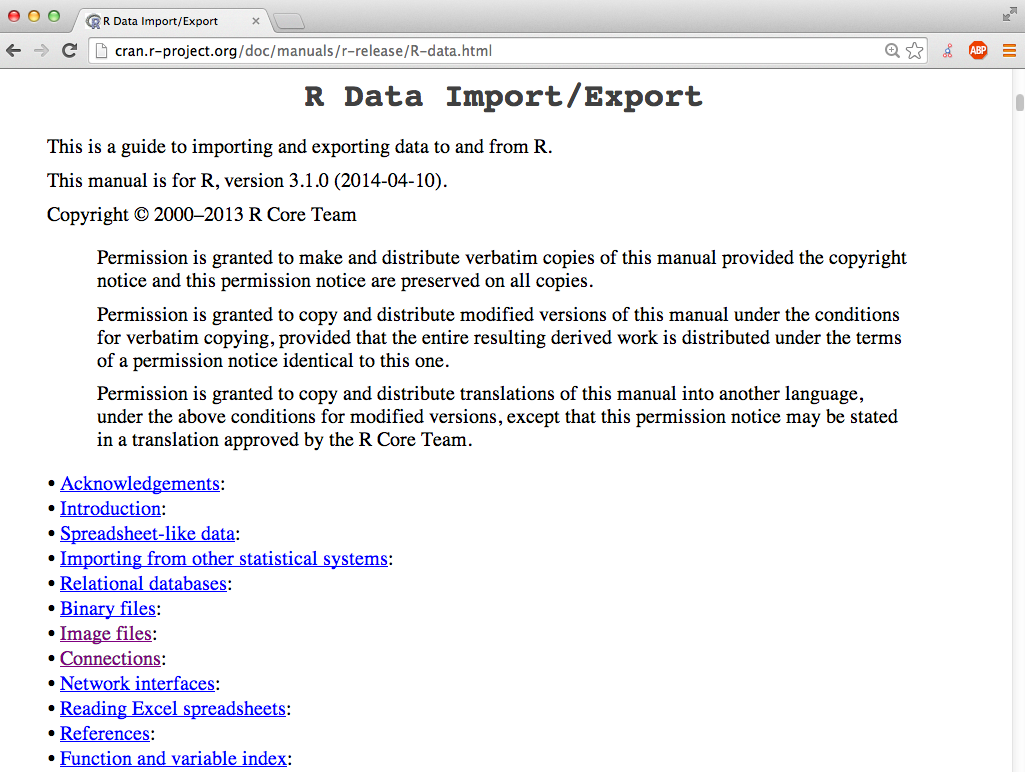
\includegraphics[width=\paperwidth]{images/R_data_import_manual.png}
            };
        \end{tikzpicture}
     \end{frame}
}

%------------------------------------------------

\begin{frame}
\frametitle{Documentation}

\begin{block}{R Data Import / Export Manual}
This is the authoritative source of information to read and learn \textit{almost all} about importing ---and exporting--- data in R:
 \begin{itemize}
  \item html version \\
  { \scriptsize \url{http://cran.r-project.org/doc/manuals/r-release/R-data.html} }
  \item pdf version \\
  { \scriptsize \url{http://cran.r-project.org/doc/manuals/r-release/R-data.pdf} }
  \end{itemize}
\end{block}

\vspace{5mm}
{ \scriptsize 
\high{Good news:} \low{pretty much everything you need to know it's there} \\
\high{Bad news:} \low{it is not beginner friendly =(}
}

\end{frame}

%------------------------------------------------

\begin{frame}
\frametitle{Basics First}

R is equipped with a set of handy functions that allow us to read a wide range of data files

\bigskip

The trick to use those functions depends on the format of the data we want to read, and the way R handles the imported values:
\begin{itemize}
 \item what type of objets \low{(eg \code{vector}, \code{list}, \code{data.frame})} 
 \item what kind of modes \low{(eg \code{character}, \code{numeric}, \code{factor})}
\end{itemize}

\end{frame}

%------------------------------------------------

\begin{frame}
\frametitle{Basics First (con't)}

\begin{columns}[t]
\begin{column}{0.2\textwidth}
%--- empty space ---%
\end{column}
\begin{column}{0.6\textwidth}

\begin{block}{Fundamentals}
Let's start with the basic reading functions and some R technicalities
 \begin{itemize}
  \item \highcode{scan()}
  \item \highcode{readLines()}
  \item \highcode{connections}
 \end{itemize}
\end{block}

\end{column}
\begin{column}{0.1\textwidth}
%--- empty space ---%
\end{column}
\end{columns}

\end{frame}

%------------------------------------------------

\begin{frame}
\frametitle{Conceptual Diagram}

\begin{center}
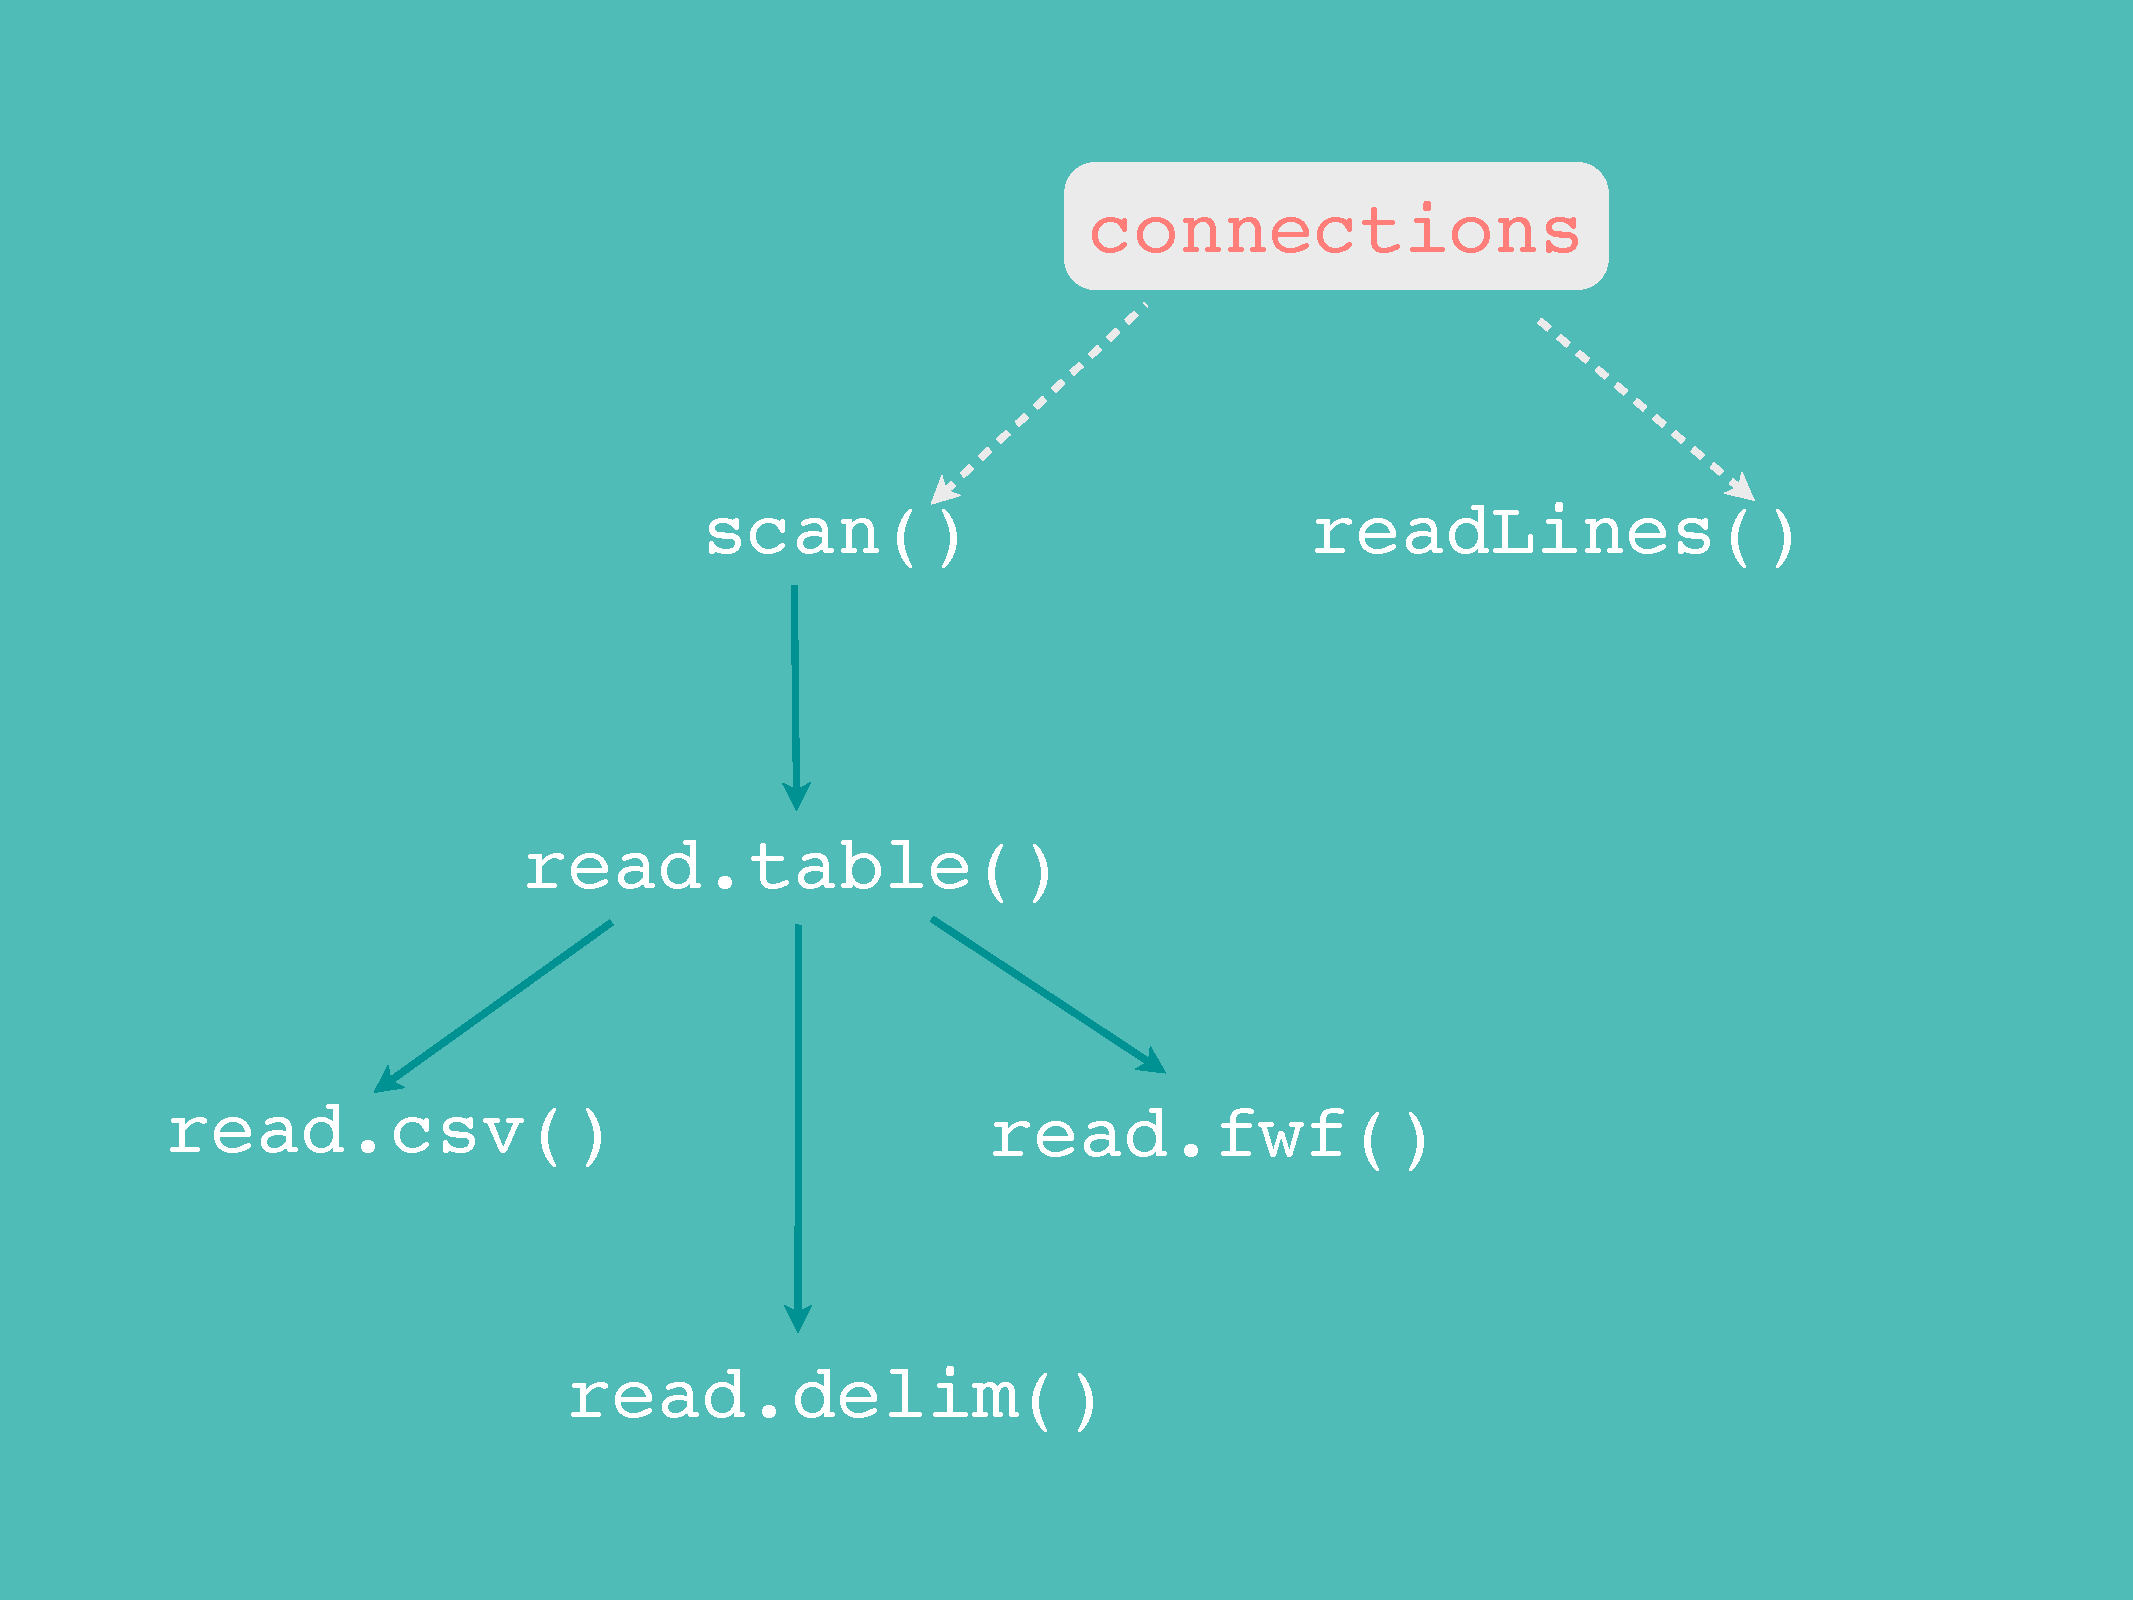
\includegraphics[width=8cm]{images/read_functions.pdf}
\end{center}

\end{frame}

%------------------------------------------------

\begin{frame}
\frametitle{Built-in reading functions}

\begin{itemize}
 \item The primary functions to read files in R are \highcode{scan()} and \highcode{readLines()}

 \item \highcode{readLines()} is the workhorse function to read raw text in R as character strings

 \item \highcode{scan()} is a low-level function for reading data values, and it is extended by \highcode{read.table()} and its related functions

 \item When reading files, there's the special concept under the hood called R \highcode{connections} 

 \item Both \code{scan()} and \code{readLines()} take a \highcode{connection} as input
\end{itemize}

\end{frame}

%------------------------------------------------

\begin{frame}
\frametitle{Connections}

\begin{block}{R connections?}
\textbf{Connection} is the term used in R to define a mechanism for handling input (reading) and output (writing) operations. 
\end{block}

\begin{block}{What do they do?}
A \textbf{connection} is just an object that tells R to be prepared for opening a data source (eg file in local directory, or a file url) \\
See the full help documentation with: \highcode{?connections}
\end{block}

\end{frame}

%------------------------------------------------

\begin{frame}
\frametitle{Types of Connections}

\begin{center}
 \begin{tabular}{l l}
  \multicolumn{2}{c}{\textcolor{turquoise}{Functions to create connections}} \\
  \hline
  Function & Input \\
  \hline
  \code{file()} & path to the file to be opened or complete URL \\
  \code{url()} & a complete URL \\
  \code{gzfile()} & path to a file compressed by \code{gzip} \\
  \code{bzfile()} & path to a file compressed by \code{bzip2} \\
  \code{xzfile()} & path to a file compressed by \code{xz} \\
  \code{unz()} & path to the zip file with \code{.zip} extension \\
  \code{pipe()} & command line to be piped to or from \\
  \code{fifo()} & path of the fifo \\
  \hline
 \end{tabular}
\end{center}

\vspace{3mm}
{\footnotesize \high{By default, creating a connection does not open the connection. But they may be opened with the argument \code{open} }
}
\end{frame}

%------------------------------------------------

\begin{frame}
\frametitle{Connections (con't)}

\begin{block}{Usefulness}
Connections provide a \textbf{means to have more control} over the way R will ``comunicate'' with the resources to be read (or written).
\end{block}

\begin{block}{Keep in mind}
Most of the times you don't need to use or worry about connections. However, you should know that they can play an important role behind the built-in fuctions to read data in R.
\end{block}

\end{frame}

%------------------------------------------------

\begin{frame}
\frametitle{Important Connections}

\begin{block}{\code{file()}}
The most commonly used connection is \highcode{file()}, which is used by most reading functions (to open a local file for reading or writing data).
\end{block}

\begin{block}{\code{url()} }
Because we're interested in getting data from the web, the one connection that becomes a protagonist is the \highcode{url()} connection.
\end{block}

\end{frame}

%------------------------------------------------

\begin{frame}[fragile]
\frametitle{Connection for the web}

\begin{block}{Using \code{url()}}
 \begin{verbatim}
url(description, open = "", blocking = TRUE,
    encoding = getOption("encoding"))
 \end{verbatim}
\end{block}

The main input for \highcode{url()} is the \highcode{description} which has to be a complete URL, including scheme such as \code{http://}, \code{ftp://}, or \code{file://}

\end{frame}

%------------------------------------------------

\begin{frame}[fragile]
\frametitle{Example of \code{url} connection}

For instance, let's create a connection to the R homepage:
\begin{knitrout}\tiny
\definecolor{shadecolor}{rgb}{1, 1, 1}\color{fgcolor}\begin{kframe}
\begin{alltt}
\hlcom{# creating a url connection to the R homepage}
\hlstd{r_home} \hlkwb{=} \hlkwd{url}\hlstd{(}\hlstr{"http://www.r-project.org/"}\hlstd{)}

\hlcom{# what's in r_home}
\hlstd{r_home}
\end{alltt}
\begin{verbatim}
##                 description                       class 
## "http://www.r-project.org/"                       "url" 
##                        mode                        text 
##                         "r"                      "text" 
##                      opened                    can read 
##                    "closed"                       "yes" 
##                   can write 
##                        "no"
\end{verbatim}
\begin{alltt}
\hlcom{# is open?}
\hlkwd{isOpen}\hlstd{(r_home)}
\end{alltt}
\begin{verbatim}
## [1] FALSE
\end{verbatim}
\end{kframe}
\end{knitrout}

{\scriptsize \high{Note that we are just defining a connection. By default, the connection does not open anything}}

\end{frame}

%------------------------------------------------

\begin{frame}
\frametitle{About Connections}

\begin{block}{Should we care?}
 \begin{itemize}
  \item Again, most of the times we don't need to explicitly use \highcode{url()}. 
  \item Connections can be used anywhere a file name could be passed to functions like \highcode{scan()} or \highcode{read.table()}. 
  \item Usually, the reading functions ---eg \code{readLines()}, \code{read.table()}, \code{read.csv()}--- will take care of the URL connection for us.
  \item However, there may be occassions in which we will need to specify a \code{url()} connection.
 \end{itemize}
\end{block}

\end{frame}

%------------------------------------------------

\begin{frame}
 \begin{center}
  \Huge{\textcolor{mandarina}{Reading Text}}
 \end{center}
\end{frame}

%------------------------------------------------

\begin{frame}
\frametitle{Objective}

\begin{columns}[t]
\begin{column}{0.1\textwidth}
%--- empty space ---%
\end{column}
\begin{column}{0.8\textwidth}

\begin{block}{Reading Text Files As Text}
In this section we'll talk about reading text files with the purpose of importing their contents as \textit{raw text} (ie character strings) in R.
\end{block}

\end{column}
\begin{column}{0.1\textwidth}
%--- empty space ---%
\end{column}
\end{columns}

\end{frame}

%------------------------------------------------

\begin{frame}
\frametitle{About Text Files}

\begin{quotation}
``In computer literature, there is often a distinction made between text files and binary files. That distinction is somewhat misleading ---every file is binary in the sense that it consists of 0s and 1s. Let's take the term text files to mean a file that consists mainly of ASCII characters ... and that uses newline characters to give the humans the perception of lines.''
\end{quotation}

{\footnotesize 
\hspace{8mm} \high{Norman Matloff (2011)} \\
\hspace{8mm} \low{The Art of R Programming}
}

\end{frame}

%------------------------------------------------

\begin{frame}
\frametitle{About Text Files}

Some considerations so we can all be on the same page:
\begin{itemize}
 \item By \high{text files} we mean \textit{plain text files} \\
 \item \textit{Plain text} as an umbrella term for any file that is in a human-readable form \low{(eg \code{.txt, .csv, .xml, .html})}
 \item Text files stored as a sequence of characters 
 \item Each character stored as a single byte of data
 \item Data is arranged in rows, with several values stored on each row
 \item Text files that can be read and manipulated with a text editor
\end{itemize}

\end{frame}

%------------------------------------------------

\begin{frame}
\frametitle{Reading Text Functions}

\begin{block}{Functions for reading text}
\begin{itemize}
 \item \highcode{readLines()} is the main function to read text files as \textit{raw text} in R
 \item \highcode{scan()} is another function that can be used to read text files. It is more generic and low-level but we can specify some of its parameters to import content as text
\end{itemize}
\end{block}

\end{frame}

%------------------------------------------------

\begin{frame}
\frametitle{About \code{readLines()}}

\begin{block}{Function \code{readLines()}}
\begin{itemize}
 \item \highcode{readLines()} is the workhorse function to read text files as \textit{raw text} in R

 \item The main input is the file to be read, either specified with a \highcode{connection} or with the file name 

\item \highcode{readLines()} treats each line as a string, and it returns a character vector

 \item The output vector will contain as many elements as number of lines in the read file
\end{itemize}
\end{block}

\end{frame}

%------------------------------------------------

\begin{frame}[fragile]
\frametitle{readLines()}

\begin{block}{Using \code{readLines()}}
 \begin{verbatim}
readLines(con = stdin(), n = -1L, ok = TRUE, 
          warn = TRUE, encoding = "unknown")
 \end{verbatim}
\end{block}

\begin{itemize}
 \item \highcode{con} a connection, which in our case will be a complete URL
 \item \highcode{n} the number of lines to read
 \item \highcode{ok} whether to reach the end of the connection
 \item \highcode{warn} warning if there is no End-Of-Line
 \item \highcode{encoding} types of encoding for input strings
\end{itemize}

\end{frame}

%------------------------------------------------

{ % all template changes are local to this group.
    \setbeamertemplate{navigation symbols}{}
    \begin{frame}[plain]
    \frametitle{Moby Dick}
        \begin{tikzpicture}[remember picture,overlay]
            \node[at=(current page.center)] {
                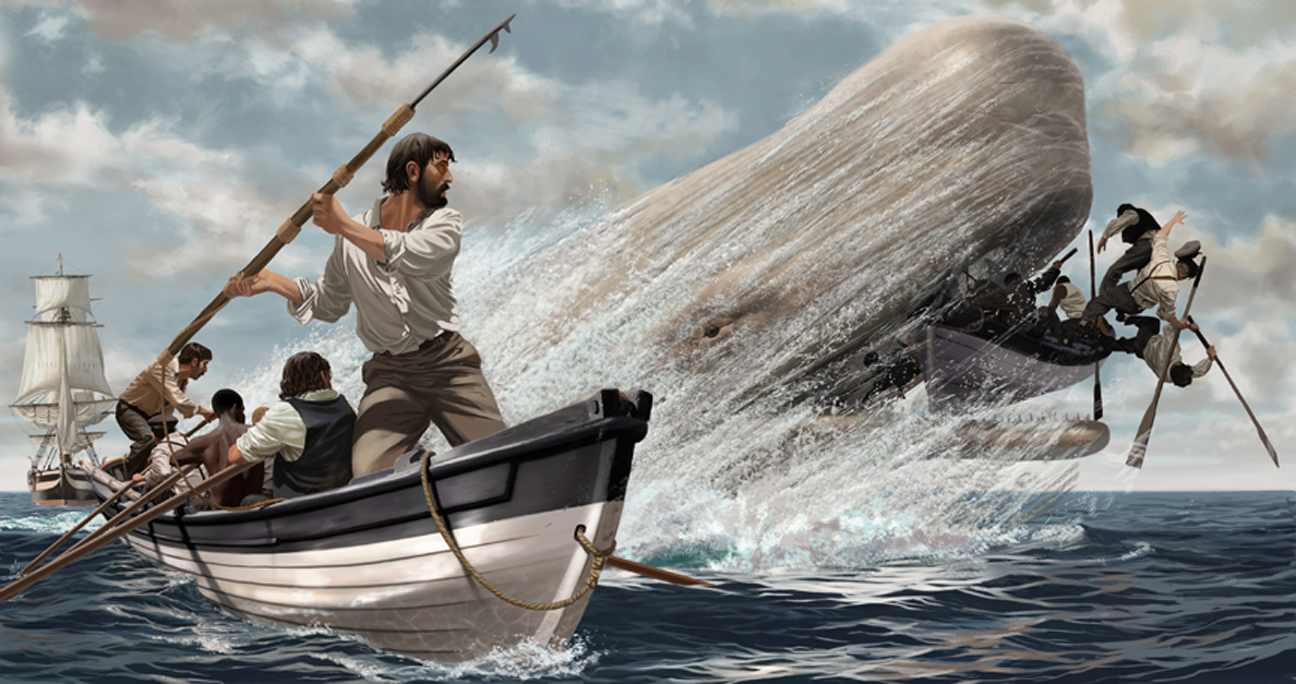
\includegraphics[width=\paperwidth]{images/moby_dick.jpg}
            };
        \end{tikzpicture}
     \end{frame}
}

%------------------------------------------------

\begin{frame}[fragile]
\frametitle{Example}

\begin{block}{Project Gutenberg}
A great collection of texts are available from the \textbf{Project Gutenberg} which has a catalog of more than 25,000 free online books: \\
{ \footnotesize \url{http://www.gutenberg.org}}
\end{block}

\begin{block}{Moby Dick}
Let's consider the famous novel \textbf{Moby Dick} by Herman Melville. 
A plain text file of Moby Dick can be found at: \\
{ \footnotesize \url{http://www.gutenberg.org/ebooks/2701.txt.utf-8}}
\end{block}

\end{frame}

%------------------------------------------------

\begin{frame}
\frametitle{Moby Dick text file}

\url{http://www.gutenberg.org/ebooks/2701.txt.utf-8}

\begin{center}
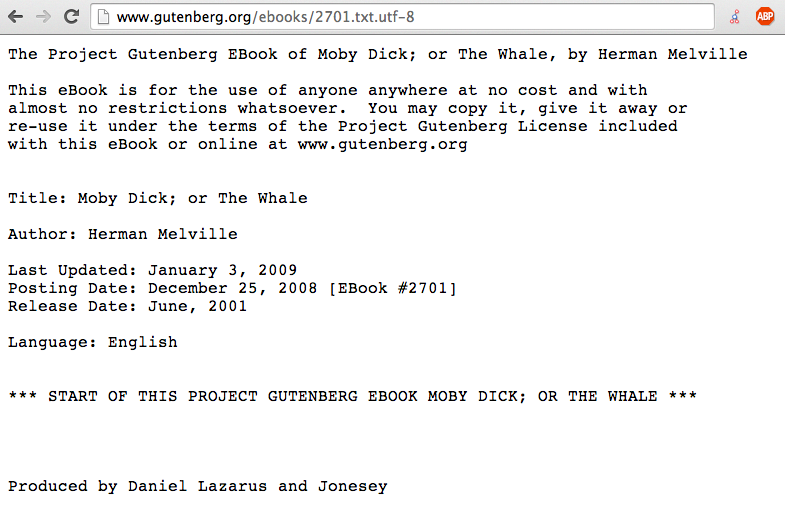
\includegraphics[width=8cm]{images/moby_dick_book.png}
\end{center}

\end{frame}

%------------------------------------------------

\begin{frame}[fragile]
\frametitle{Reading Raw text}

Here's how you could read the first 500 lines of cotent with \highcode{readLines()}

\begin{knitrout}\tiny
\definecolor{shadecolor}{rgb}{1, 1, 1}\color{fgcolor}\begin{kframe}
\begin{alltt}
\hlcom{# url of Moby Dick (project Gutenberg)}
\hlstd{moby_url} \hlkwb{=} \hlkwd{url}\hlstd{(}\hlstr{"http://www.gutenberg.org/ebooks/2701.txt.utf-8"}\hlstd{)}

\hlcom{# reading the content (first 500 lines)}
\hlstd{moby_dick} \hlkwb{=} \hlkwd{readLines}\hlstd{(moby_url,} \hlkwc{n} \hlstd{=} \hlnum{500}\hlstd{)}
\end{alltt}
\end{kframe}
\end{knitrout}



\begin{knitrout}\tiny
\definecolor{shadecolor}{rgb}{1, 1, 1}\color{fgcolor}\begin{kframe}
\begin{alltt}
\hlcom{# first five lines}
\hlstd{moby_dick[}\hlnum{1}\hlopt{:}\hlnum{5}\hlstd{]}
\end{alltt}
\begin{verbatim}
## [1] "The Project Gutenberg EBook of Moby Dick; or The Whale, by Herman Melville"
## [2] ""                                                                          
## [3] "This eBook is for the use of anyone anywhere at no cost and with"          
## [4] "almost no restrictions whatsoever.  You may copy it, give it away or"      
## [5] "re-use it under the terms of the Project Gutenberg License included"
\end{verbatim}
\end{kframe}
\end{knitrout}

{\footnotesize \high{Note that each line read is stored as an element in the character vector \code{moby\_dick}}}

\end{frame}

%------------------------------------------------

\begin{frame}[fragile]
\frametitle{Goot to Know}

\begin{block}{Terms of Service}
Some times, reading data directly from a website may be against the \high{terms of use} of the site.
\end{block}

\begin{block}{Web Politeness}
When you're reading (and ``playing'' with) content from a web page, make a local copy as a courtesy to the owner of the web site so you don't overload their server by constantly rereading the page. To make a copy from inside of R, look at the \highcode{download.file()} function. 
\end{block}

\end{frame}

%------------------------------------------------

\begin{frame}[fragile]
\frametitle{Download Moby Dick}

\begin{block}{Downloading}
It is good advice to download a copy of the file to your computer, and then play with it. 

\bigskip

Let's use \highcode{download.file()} to save a copy in our working directory. In this case we create the file \highcode{mobydick.txt}

\begin{knitrout}\tiny
\definecolor{shadecolor}{rgb}{1, 1, 1}\color{fgcolor}\begin{kframe}
\begin{alltt}
\hlcom{# download a copy in the working directory}
\hlkwd{download.file}\hlstd{(}\hlstr{"http://www.gutenberg.org/cache/epub/2701/pg2701.txt"}\hlstd{,}
              \hlstr{"mobydick.txt"}\hlstd{)}
\end{alltt}
\end{kframe}
\end{knitrout}
\end{block}

\end{frame}

%------------------------------------------------

\begin{frame}[fragile]
\frametitle{Abut scan()}

\begin{block}{Function \code{scan()}}
Another very useful function that we can use to read text is \highcode{scan()}. By default, \code{scan()} expects to read numeric values, but we can change this behavior with the argument \highcode{what}

{\footnotesize
\begin{verbatim}
scan(file = "", what = double(), nmax = -1, n = -1, sep = "",
     quote = if(identical(sep, "\n")) "" else "'\"", dec = ".",
     skip = 0, nlines = 0, na.strings = "NA",
     flush = FALSE, fill = FALSE, strip.white = FALSE,
     quiet = FALSE, blank.lines.skip = TRUE, multi.line = TRUE,
     comment.char = "", allowEscapes = FALSE,
     fileEncoding = "", encoding = "unknown", text)
 \end{verbatim}
}

\end{block}

\end{frame}

%------------------------------------------------

\begin{frame}[fragile]
\frametitle{Function scan() (con't)}

\begin{block}{Some \code{scan()} arguments}
\begin{itemize}
 \item \highcode{file} the file name or a connection
 \item \highcode{what} type of data to be read
 \item \highcode{n} maximum number of data values to read
 \item \highcode{sep} type of separator
 \item \highcode{skip} number of lines to skip before reading values
 \item \highcode{nlines} maximum number of lines to be read
\end{itemize}
\end{block}

\end{frame}

%------------------------------------------------

\begin{frame}
\frametitle{Moby Dick Chapter 1}

Chapter 1 starting at line 536. \\
How do we get the first lines of that chapter?
\begin{center}
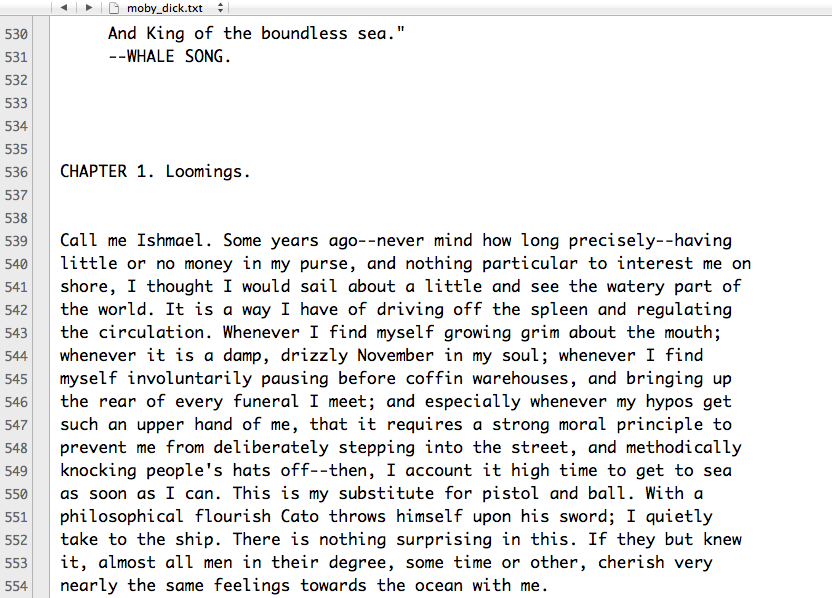
\includegraphics[width=8cm]{images/moby_dick_535.png}
\end{center}

\end{frame}

%------------------------------------------------

\begin{frame}[fragile]
\frametitle{Reading Some Lines}

\begin{block}{Let's make it more interesting}
If we want to read just a pre-specified number of lines, we have to loop over the file lines and read the content with \highcode{scan()}. For instance, let's skip the first 535 lines, and then read the following 10 lines of Chapter 1

\begin{knitrout}\tiny
\definecolor{shadecolor}{rgb}{1, 1, 1}\color{fgcolor}\begin{kframe}
\begin{alltt}
\hlcom{# empty vector to store results}
\hlstd{moby_dick_chap1} \hlkwb{=} \hlkwd{rep}\hlstd{(}\hlstr{""}\hlstd{,} \hlnum{10}\hlstd{)}

\hlcom{# number of lines to skip until Chapter 1}
\hlstd{skip} \hlkwb{=} \hlnum{535}

\hlcom{# reading 10 lines (line-by-line using scan)}
\hlkwa{for} \hlstd{(i} \hlkwa{in} \hlnum{1L}\hlopt{:}\hlnum{10}\hlstd{) \{}
  \hlstd{one_line} \hlkwb{=} \hlkwd{scan}\hlstd{(}\hlstr{"mobydick.txt"}\hlstd{,} \hlkwc{what} \hlstd{=} \hlstr{""}\hlstd{,} \hlkwc{skip} \hlstd{= skip,} \hlkwc{nlines} \hlstd{=} \hlnum{1}\hlstd{)}
  \hlcom{# pasting the contents in one_line}
  \hlstd{moby_dick_chap1[i]} \hlkwb{=} \hlkwd{paste}\hlstd{(one_line,} \hlkwc{collapse} \hlstd{=} \hlstr{" "}\hlstd{)}
  \hlstd{skip} \hlkwb{=} \hlstd{skip} \hlopt{+} \hlnum{1}
\hlstd{\}}
\end{alltt}
\end{kframe}
\end{knitrout}



{\scriptsize \high{Note that we are using \code{paste()} to join (collapse) all the scanned values in \code{one\_line}}}
\end{block}

\end{frame}

%------------------------------------------------

\begin{frame}[fragile]
\frametitle{Reading Some Lines (con't)}

\begin{knitrout}\tiny
\definecolor{shadecolor}{rgb}{1, 1, 1}\color{fgcolor}\begin{kframe}
\begin{alltt}
\hlcom{# lines 536-545}
\hlstd{moby_dick_chap1}
\end{alltt}
\begin{verbatim}
##  [1] "CHAPTER 1. Loomings."                                                    
##  [2] ""                                                                        
##  [3] ""                                                                        
##  [4] "Call me Ishmael. Some years ago--never mind how long precisely--having"  
##  [5] "little or no money in my purse, and nothing particular to interest me on"
##  [6] "shore, I thought I would sail about a little and see the watery part of" 
##  [7] "the world. It is a way I have of driving off the spleen and regulating"  
##  [8] "the circulation. Whenever I find myself growing grim about the mouth;"   
##  [9] "whenever it is a damp, drizzly November in my soul; whenever I find"     
## [10] "myself involuntarily pausing before coffin warehouses, and bringing up"
\end{verbatim}
\end{kframe}
\end{knitrout}

\end{frame}

%------------------------------------------------

\begin{frame}[fragile]
\frametitle{Reading an HTML file}

\begin{block}{HTML File}
Our third example involves reading the contents of an html file. We're just illustrating how to import html content as raw text in R. \\
\low{(We are not \textit{parsing} html; we'll see that topic in the next lecture)}
\end{block}

\begin{block}{Egyptian Skulls}
Let's consider the file containing information about the Egyptian Skulls data set by Thomson \textit{et al}: \\
{ \footnotesize \url{http://lib.stat.cmu.edu/DASL/Datafiles/EgyptianSkulls.html}}
\end{block}

\end{frame}

%------------------------------------------------

\begin{frame}
\frametitle{HTML File}

{\footnotesize \url{http://lib.stat.cmu.edu/DASL/Datafiles/EgyptianSkulls.html}}

\begin{center}
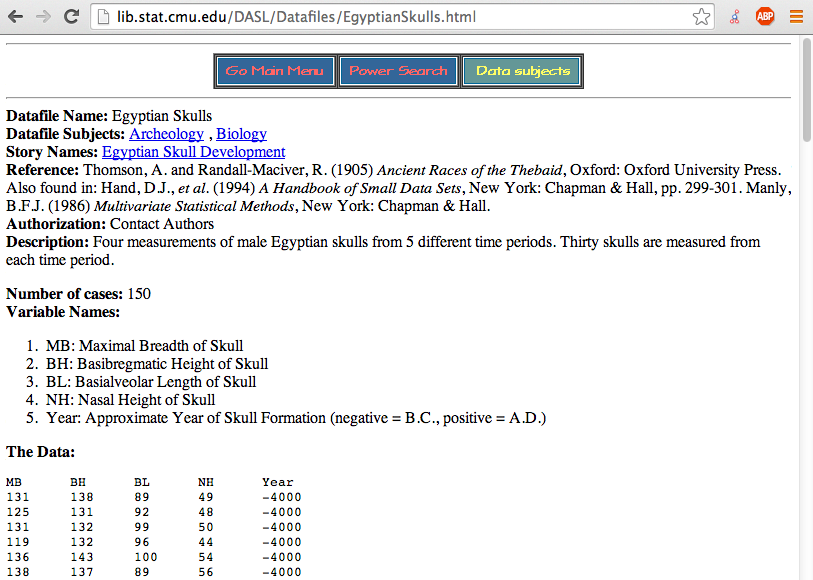
\includegraphics[width=8cm]{images/skulls_data.png}
\end{center}

\end{frame}

%------------------------------------------------

\begin{frame}[fragile]
\frametitle{Skulls Data}

To read the html content we use \highcode{readLines()}

\begin{knitrout}\tiny
\definecolor{shadecolor}{rgb}{1, 1, 1}\color{fgcolor}\begin{kframe}
\begin{alltt}
\hlcom{# read html file content as a string vector}
\hlstd{skulls} \hlkwb{=} \hlkwd{readLines}\hlstd{(}\hlstr{"http://lib.stat.cmu.edu/DASL/Datafiles/EgyptianSkulls.html"}\hlstd{)}
\end{alltt}
\end{kframe}
\end{knitrout}

\begin{knitrout}\tiny
\definecolor{shadecolor}{rgb}{1, 1, 1}\color{fgcolor}\begin{kframe}
\begin{alltt}
\hlkwd{head}\hlstd{(skulls,} \hlkwc{n} \hlstd{=} \hlnum{10}\hlstd{)}
\end{alltt}
\begin{verbatim}
##  [1] "<TITLE>Egyptian Skulls Datafile</TITLE>"                                                                                                                                                                                                                                                                                                                                                                                                                                                                                                                                                                                                                                                                                       
##  [2] ""                                                                                                                                                                                                                                                                                                                                                                                                                                                                                                                                                                                                                                                                                                                              
##  [3] ""                                                                                                                                                                                                                                                                                                                                                                                                                                                                                                                                                                                                                                                                                                                              
##  [4] "<hr size=2><center><table border=1 cellpadding=0 cellspacing=0><tr><td align=center><table border=1 cellpadding=1 cellspacing=0><tr><td><A HREF=\"../DataArchive.html\"><IMG SRC=\"../InlineImages/mainmenu.gif\" alt=\"Go to Main Menu\"></a></td></tr></table></td><td align=center><table border=1 cellpadding=1 cellspacing=0><tr><td><A HREF=\"/cgi-bin/dasl.cgi\"><IMG SRC=\"../InlineImages/powersearchsmall.gif\" alt=\"Go to Power Search\"></a></td></tr></table></td><td align=center><table border=1 cellpadding=1 cellspacing=0><tr><td><A HREF=\"../allsubjects.html\"><IMG SRC=\"../InlineImages/allsubjects.gif\" alt=\"Go to Datafile Subjects\"></a></td></tr></table></td></tr></table></center><hr size=2>"
##  [5] "<B><DT>Datafile Name:</B>   Egyptian Skulls"                                                                                                                                                                                                                                                                                                                                                                                                                                                                                                                                                                                                                                                                                   
##  [6] "<B><DT>Datafile Subjects:</B>   <dsubjects>"                                                                                                                                                                                                                                                                                                                                                                                                                                                                                                                                                                                                                                                                                   
##  [7] "<A HREF=\"/cgi-bin/dasl.cgi?query=Archeology&submit=Search&metaname=dsubjects&sort=swishrank\">Archeology</A>"                                                                                                                                                                                                                                                                                                                                                                                                                                                                                                                                                                                                                 
##  [8] ", "                                                                                                                                                                                                                                                                                                                                                                                                                                                                                                                                                                                                                                                                                                                            
##  [9] ""                                                                                                                                                                                                                                                                                                                                                                                                                                                                                                                                                                                                                                                                                                                              
## [10] "<A HREF=\"/cgi-bin/dasl.cgi?query=Biology&submit=Search&metaname=dsubjects&sort=swishrank\">Biology</A>"
\end{verbatim}
\end{kframe}
\end{knitrout}

\end{frame}

%------------------------------------------------

\begin{frame}
 \begin{center}
  \Huge{\textcolor{mandarina}{Reading Tabular Data}}
 \end{center}
\end{frame}

%------------------------------------------------

\begin{frame}[fragile]
\frametitle{About Tabular Data}

\begin{block}{Tables}
R is great for reading data in tabular \low{(spreadsheet-like)} format.

\bigskip
Tabular data, also known as rectangular data, are typically text files \low{(ie can be read and manipulated with a text editor)}

\bigskip
The conventional form is data values that can be seen as an array of rows and columns
\end{block}

\end{frame}

%------------------------------------------------

\begin{frame}[fragile]
\frametitle{Tabular Data File Formats}

\begin{block}{Two main formats}
 \begin{itemize}
  \item delimited formats
  \item fixed-width formats
 \end{itemize}
\end{block}

\begin{block}{Delimited}
In a delimited format, values within a row are separated by a special character, or delimiter.
\end{block}

\begin{block}{Fixed-Width}
In a fixed-width format, each value is allocated a fixed number of characters within every row.
\end{block}

\end{frame}

%------------------------------------------------



%------------------------------------------------

\begin{frame}[fragile]
\frametitle{Data Table Toy Example}

\begin{center}
\textcolor{turquoise}{Imagine we have some tabular data}
\end{center}

\begin{center}
 \begin{tabular}{l l l l l}
  \hline
  Name & Gender & Homeland & Born & Jedi \\
  \hline
  Anakin & male & Tatooine & 41.9BBY & yes \\  
  Amidala & female & Naboo & 46BBY & no \\
  Luke & male & Tatooine & 19BBY & yes \\
  Leia & female & Alderaan & 19BBY & no \\
  Obi-Wan & male & Stewjon & 57BBY & yes \\
  Han & male & Corellia & 29BBY & no \\
  Palpatine & male & Naboo & 82BBY & no \\
  R2-D2 & unknown & Naboo & 33BBY & no \\
  \hline
 \end{tabular}
\end{center}

\end{frame}

%------------------------------------------------

\begin{frame}[fragile]
\frametitle{Data table formats}

\begin{columns}[t]
\begin{column}{0.35\textwidth}
\high{space delimited}
{\tiny \begin{verbatim}
Name Gender Homeworld Born Jedi
Anakin male Tatooine 41.9BBY yes  
Amidala female Naboo 46BBY no
Luke male Tatooine 19BBY yes
Leia female Alderaan 19BBY no
Obi-Wan male Stewjon 57BBY yes
Han male Corellia 29BBY no
Palpatine male Naboo 82BBY no
R2-D2 unknown Naboo 33BBY no
\end{verbatim}}
\end{column}
\begin{column}{0.4\textwidth}
\high{tab delimited}
{\tiny \begin{verbatim}
Name  Gender  Homeworld  Born  Jedi
Anakin  male  Tatooine  41.9BBY yes	
Amidala female  Naboo 46BBY no
Luke  male  Tatooine  19BBY yes
Leia  female  Alderaan  19BBY no
Obi-Wan male  Stewjon 57BBY yes
Han male  Corellia  29BBY no
Palpatine male  Naboo 82BBY no
R2-D2 unknown	Naboo 33BBY no
\end{verbatim}}
\end{column}
\end{columns}

\vspace{5mm}

\begin{columns}[t]
\begin{column}{0.35\textwidth}
\high{comma delimited}
{\tiny \begin{verbatim}
Name,Gender,Homeworld,Born,Jedi
Anakin,male,Tatooine,41.9BBY,yes  
Amidala,female,Naboo,46BBY,no
Luke,male,Tatooine,19BBY,yes
Leia,female,Alderaan,19BBY,no
Obi-Wan,male,Stewjon,57BBY,yes
Han,male,Corellia,29BBY,no
Palpatine,male,Naboo,82BBY,no
R2-D2,unknown,Naboo,33BBY,no
\end{verbatim}}
\end{column}
\begin{column}{0.4\textwidth}
\high{Fixed width}
{\tiny \begin{verbatim}
Name      Gender  Homeworld Born     Jedi
Anakin    male    Tatooine  41.9BBY  yes  
Amidala   female  Naboo     46BBY    no
Luke      male    Tatooine  19BBY    yes
Leia      female  Alderaan  19BBY    no
Obi-Wan   male    Stewjon   57BBY    yes
Han       male    Corellia  29BBY    no
Palpatine male    Naboo     82BBY    no
R2-D2     unknown Naboo     33BBY    no
\end{verbatim}}
\end{column}
\end{columns}

\end{frame}

%------------------------------------------------

\begin{frame}[fragile]
\frametitle{Functions}

\begin{block}{Main functions}
\begin{itemize}
 \item \highcode{scan()} reads data values (one by one)
 \item \highcode{read.table()} main function for reading tabular data
 \item \highcode{read.csv()} convenient wraper of \code{read.table()} designed for reading \textit{comma separated values} (CSV) files
 \item \highcode{read.delim()} wrapper of \code{read.table()} for any delimited file format
 \item \highcode{read.fwf()} designed for reading files with fixed width 
 separated values
\end{itemize}
\end{block}

\end{frame}

%------------------------------------------------

\begin{frame}[fragile]
\frametitle{Taxon Data}

\begin{block}{The R Book}
Example from \textbf{The R Book} by Michael Crawley \\
{\scriptsize \url{http://www.bio.ic.ac.uk/research/mjcraw/therbook/}}
\end{block}

\begin{center}
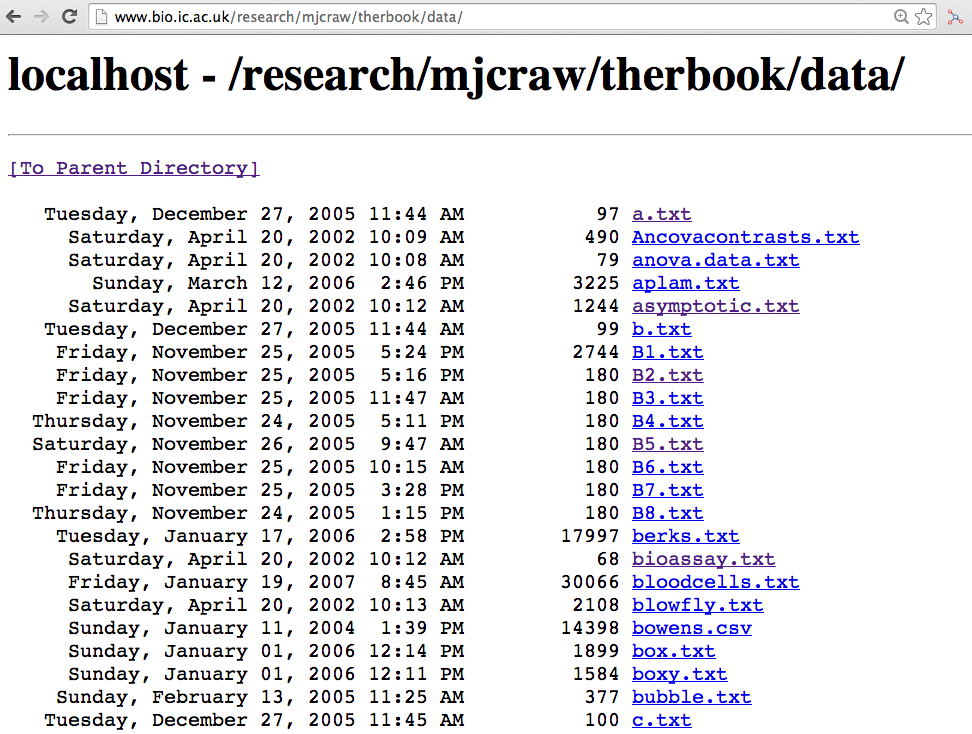
\includegraphics[width=7cm]{images/rbook_files.png}
\end{center}

\end{frame}

%------------------------------------------------

\begin{frame}
\frametitle{Taxon Data}

Taxon Data (from The R Book) \\
{\scriptsize \url{http://www.bio.ic.ac.uk/research/mjcraw/therbook/data/taxon.txt}}
\begin{center}
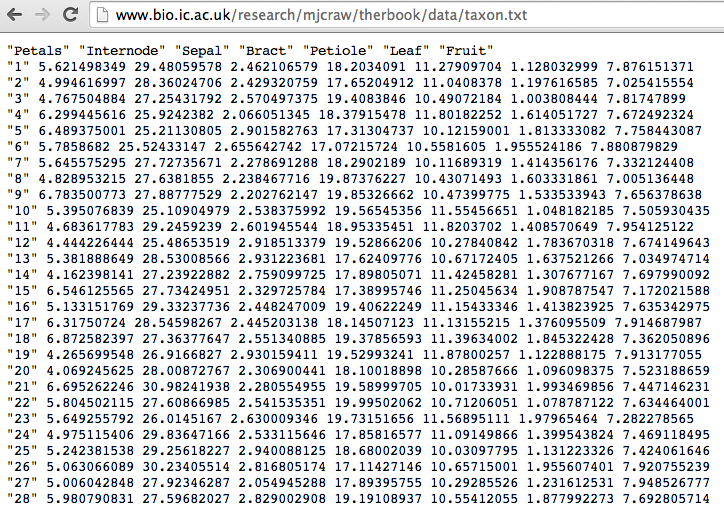
\includegraphics[width=8cm]{images/taxon_data.png}
\end{center}

\end{frame}

%------------------------------------------------

\begin{frame}[fragile]
\frametitle{Taxon Data}

Let's read the data \highcode{"taxon"}

\begin{knitrout}\tiny
\definecolor{shadecolor}{rgb}{1, 1, 1}\color{fgcolor}\begin{kframe}
\begin{alltt}
\hlcom{# url of taxon data}
\hlstd{taxon_url} \hlkwb{=} \hlstr{"http://www.bio.ic.ac.uk/research/mjcraw/therbook/data/taxon.txt"}

\hlcom{# import data in R}
\hlstd{taxon} \hlkwb{=} \hlkwd{read.table}\hlstd{(taxon_url,} \hlkwc{header} \hlstd{=} \hlnum{TRUE}\hlstd{,} \hlkwc{row.names} \hlstd{=} \hlnum{1}\hlstd{)}
\end{alltt}
\end{kframe}
\end{knitrout}

\begin{knitrout}\tiny
\definecolor{shadecolor}{rgb}{1, 1, 1}\color{fgcolor}\begin{kframe}
\begin{alltt}
\hlkwd{head}\hlstd{(taxon)}
\end{alltt}
\begin{verbatim}
##     Petals Internode    Sepal    Bract  Petiole     Leaf    Fruit
## 1 5.621498  29.48060 2.462107 18.20341 11.27910 1.128033 7.876151
## 2 4.994617  28.36025 2.429321 17.65205 11.04084 1.197617 7.025416
## 3 4.767505  27.25432 2.570497 19.40838 10.49072 1.003808 7.817479
## 4 6.299446  25.92424 2.066051 18.37915 11.80182 1.614052 7.672492
## 5 6.489375  25.21131 2.901583 17.31305 10.12159 1.813333 7.758443
## 6 5.785868  25.52433 2.655643 17.07216 10.55816 1.955524 7.880880
\end{verbatim}
\end{kframe}
\end{knitrout}

\end{frame}

%------------------------------------------------

\begin{frame}[fragile]
\frametitle{Iris Example}

\begin{block}{Iris Data}
Data set \highcode{"iris"} from UCI Machine Learning Repo \\
{\scriptsize 
\url{https://archive.ics.uci.edu/ml/machine-learning-databases/iris/iris.data}}

\begin{center}
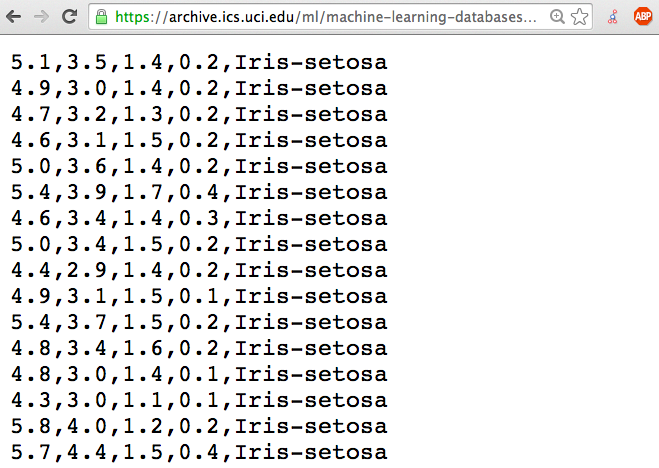
\includegraphics[width=8cm]{images/iris_data.png}
\end{center}

Example from the \textbf{UCI Machine Learning Repository} \\
{\scriptsize \url{https://archive.ics.uci.edu/ml/datasets.html}}
\end{block}

\end{frame}

%------------------------------------------------

\begin{frame}[fragile]
\frametitle{Iris Data}

\begin{block}{How do we read the data?}
If you try to simply use \code{read.csv()}, you'll be disappointed:
\begin{knitrout}\tiny
\definecolor{shadecolor}{rgb}{1, 1, 1}\color{fgcolor}\begin{kframe}
\begin{alltt}
\hlcom{# URL of data file}
\hlstd{iris_file} \hlkwb{=} \hlstr{"https://archive.ics.uci.edu/ml/machine-learning-databases/iris/iris.data"}

\hlcom{# this won't work}
\hlstd{iris_data} \hlkwb{=} \hlkwd{read.csv}\hlstd{(iris_file,} \hlkwc{header} \hlstd{=} \hlnum{FALSE}\hlstd{)}
\end{alltt}
\end{kframe}
\end{knitrout}
\end{block}

Note that the URL starts with \highcode{https://}, that means a secured connection. The solution requires some special functions:
\begin{itemize}
 \item We need to use the R package \highcode{"RCurl"} to make an \code{HTTPS} request with \highcode{getURL()}
 \item We also need to use \highcode{textConnection()} inside \highcode{read.csv()}
\end{itemize}

\end{frame}

%------------------------------------------------

\begin{frame}[fragile]
\frametitle{Reading Iris Data}

This is how to successfully read the iris data set in R:
\begin{knitrout}\tiny
\definecolor{shadecolor}{rgb}{1, 1, 1}\color{fgcolor}\begin{kframe}
\begin{alltt}
\hlcom{# URL of data file}
\hlstd{iris_file} \hlkwb{=} \hlstr{"https://archive.ics.uci.edu/ml/machine-learning-databases/iris/iris.data"}

\hlkwd{library}\hlstd{(RCurl)}
\hlstd{iris_url} \hlkwb{=} \hlkwd{getURL}\hlstd{(iris_file)}
\hlstd{iris_data} \hlkwb{=} \hlkwd{read.csv}\hlstd{(}\hlkwd{textConnection}\hlstd{(iris_url),} \hlkwc{header} \hlstd{=} \hlnum{FALSE}\hlstd{)}
\end{alltt}
\end{kframe}
\end{knitrout}

\begin{knitrout}\tiny
\definecolor{shadecolor}{rgb}{1, 1, 1}\color{fgcolor}\begin{kframe}
\begin{alltt}
\hlkwd{head}\hlstd{(iris_data)}
\end{alltt}
\begin{verbatim}
##    V1  V2  V3  V4          V5
## 1 5.1 3.5 1.4 0.2 Iris-setosa
## 2 4.9 3.0 1.4 0.2 Iris-setosa
## 3 4.7 3.2 1.3 0.2 Iris-setosa
## 4 4.6 3.1 1.5 0.2 Iris-setosa
## 5 5.0 3.6 1.4 0.2 Iris-setosa
## 6 5.4 3.9 1.7 0.4 Iris-setosa
\end{verbatim}
\end{kframe}
\end{knitrout}

\end{frame}

%------------------------------------------------

\begin{frame}[fragile]
\frametitle{Excel File Example}

\begin{block}{Excel file}
Example from \textit{Data Mining Course} by Lluis Belanche \\
{\scriptsize 
\url{http://www.lsi.upc.edu/~belanche/Docencia/mineria/mineria.html}}

\begin{center}
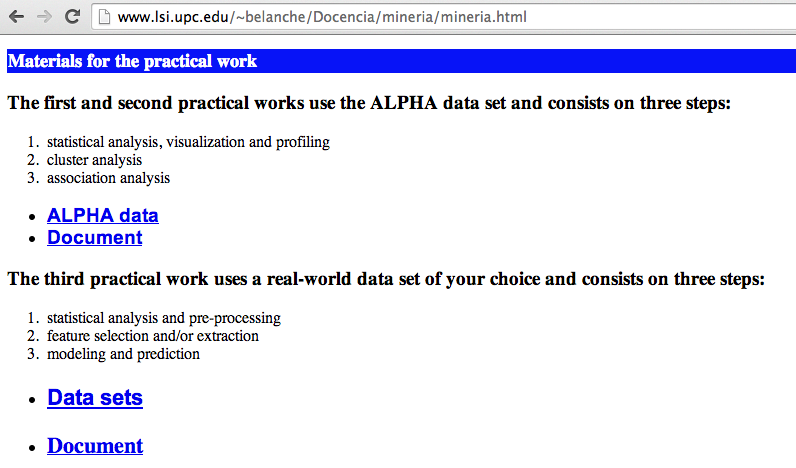
\includegraphics[width=6cm]{images/mineria_webpage.png}
\end{center}

We'll read the excel file named \code{alpha.xls} available at: \\
{\tiny 
\url{alpha_xls = "http://www.lsi.upc.edu/~belanche/Docencia/mineria/Practiques/alpha.xls"
}}
\end{block}

\end{frame}

%------------------------------------------------

\begin{frame}
\frametitle{Excel alpha data}

Alpha Data (from Data Mining course)
\begin{center}
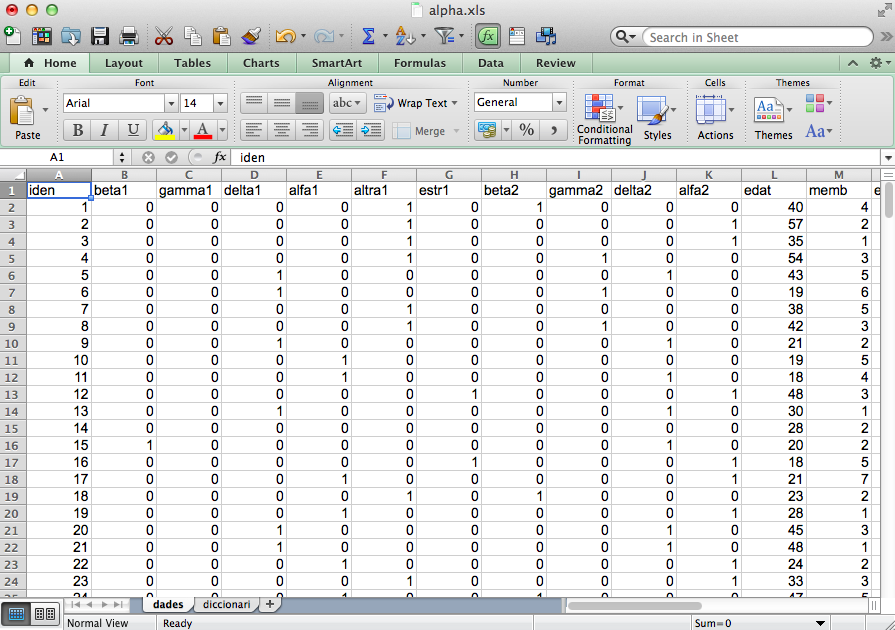
\includegraphics[width=8cm]{images/alpha_data.png}
\end{center}

\end{frame}

%------------------------------------------------



\begin{frame}[fragile]
\frametitle{Reading alpha Data}

We need to use the function \highcode{read.xls()} from the package \highcode{"gdata"} \low{(you need to have Perl installed in your machine)}
\begin{knitrout}\tiny
\definecolor{shadecolor}{rgb}{1, 1, 1}\color{fgcolor}\begin{kframe}
\begin{alltt}
\hlcom{# load package 'gdata'}
\hlkwd{library}\hlstd{(gdata)}

\hlcom{# excel file (1st worksheet named "dades")}
\hlstd{alpha_xls} \hlkwb{=} \hlstr{"http://www.lsi.upc.edu/~belanche/Docencia/mineria/Practiques/alpha.xls"}
\end{alltt}
\end{kframe}
\end{knitrout}

Count the number of sheets in excel file, and list sheet names:
\begin{knitrout}\tiny
\definecolor{shadecolor}{rgb}{1, 1, 1}\color{fgcolor}\begin{kframe}
\begin{alltt}
\hlcom{# how many sheets}
\hlkwd{sheetCount}\hlstd{(alpha_xls)}
\end{alltt}
\begin{verbatim}
## [1] 2
\end{verbatim}
\begin{alltt}
\hlcom{# names of sheets}
\hlkwd{sheetNames}\hlstd{(alpha_xls)}
\end{alltt}
\begin{verbatim}
## [1] "dades"      "diccionari"
\end{verbatim}
\end{kframe}
\end{knitrout}

\end{frame}

%------------------------------------------------

\begin{frame}[fragile]
\frametitle{Reading alpha Data}

Since the data set is in the first worksheet we use the argument \highcode{sheet = 1}:
\begin{knitrout}\tiny
\definecolor{shadecolor}{rgb}{1, 1, 1}\color{fgcolor}\begin{kframe}
\begin{alltt}
\hlcom{# import sheet 1 (dades) in R}
\hlstd{alpha_data} \hlkwb{=} \hlkwd{read.xls}\hlstd{(alpha_xls,} \hlkwc{sheet} \hlstd{=} \hlnum{1}\hlstd{)}

\hlkwd{head}\hlstd{(alpha_data)}
\end{alltt}
\begin{verbatim}
##   iden beta1 gamma1 delta1 alfa1 altra1 estr1 beta2 gamma2 delta2 alfa2 edat
## 1    1     0      0      0     0      1     0     1      0      0     0   40
## 2    2     0      0      0     0      1     0     0      0      0     1   57
## 3    3     0      0      0     0      1     0     0      0      0     1   35
## 4    4     0      0      0     0      1     0     0      1      0     0   54
## 5    5     0      0      1     0      0     0     0      0      1     0   43
## 6    6     0      0      1     0      0     0     0      1      0     0   19
##   memb estd eciv prof1 prof2 ingr
## 1    4   12    1     1     0  190
## 2    2   12    1     1     0  220
## 3    1   16    0     1     0  220
## 4    3   14    1     1     0  220
## 5    5   14    1     0     1  110
## 6    6   14    0     0     0  220
\end{verbatim}
\end{kframe}
\end{knitrout}

\end{frame}

%------------------------------------------------

\begin{frame}[fragile]
\frametitle{Google Spreadsheet}

\begin{block}{Cars2004 Data}
Example with data in Google Docs Spreadsheet \\
\begin{center}
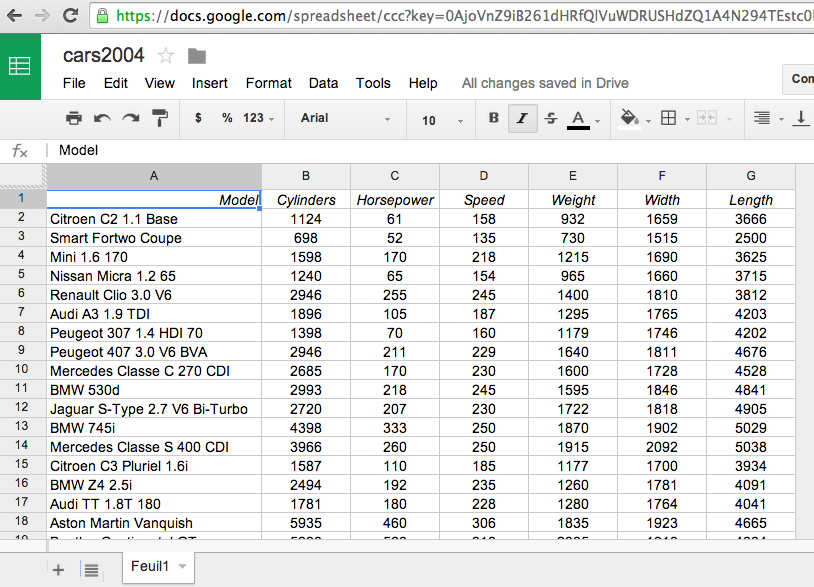
\includegraphics[width=8cm]{images/cars2004_data.png}

\scalebox{.5}{\url{https://docs.google.com/spreadsheet/ccc?key=0AjoVnZ9iB261dHRfQlVuWDRUSHdZQ1A4N294TEstc0E&usp=sharing
}}
\end{center}
\end{block}

\end{frame}

%------------------------------------------------

\begin{frame}[fragile]
\frametitle{Reading Cars2004 Google Doc}

To read data from a Google Doc Spreadsheet we need to use the R package \highcode{"RCurl"} (to connect via a secured HTTP). In addition we need to know the \textbf{publick key} of the document. Here's how to read the Cars2004 google doc:
\begin{knitrout}\tiny
\definecolor{shadecolor}{rgb}{1, 1, 1}\color{fgcolor}\begin{kframe}
\begin{alltt}
\hlcom{# load package RCurl}
\hlkwd{library}\hlstd{(RCurl)}

\hlcom{# google docs spreadsheets url}
\hlstd{google_docs} \hlkwb{=} \hlstr{"https://docs.google.com/spreadsheet/"}

\hlcom{# public key of data 'cars'}
\hlstd{cars_key} \hlkwb{=} \hlstr{"pub?key=0AjoVnZ9iB261dHRfQlVuWDRUSHdZQ1A4N294TEstc0E&output=csv"}

\hlcom{# download URL of data file}
\hlstd{cars_csv} \hlkwb{=} \hlkwd{getURL}\hlstd{(}\hlkwd{paste}\hlstd{(google_docs, cars_key,} \hlkwc{sep} \hlstd{=} \hlstr{""}\hlstd{))}

\hlcom{# import data in R (through a text connection)}
\hlstd{cars2004} \hlkwb{=} \hlkwd{read.csv}\hlstd{(}\hlkwd{textConnection}\hlstd{(cars_csv),} \hlkwc{row.names} \hlstd{=} \hlnum{1}\hlstd{,} \hlkwc{header} \hlstd{=} \hlnum{TRUE}\hlstd{)}
\end{alltt}
\end{kframe}
\end{knitrout}

\end{frame}

%------------------------------------------------

\begin{frame}[fragile]
\frametitle{Reading Cars2004 Google Doc}

\begin{knitrout}\tiny
\definecolor{shadecolor}{rgb}{1, 1, 1}\color{fgcolor}\begin{kframe}
\begin{alltt}
\hlstd{cars2004} \hlkwb{=} \hlkwd{read.csv}\hlstd{(mycars,} \hlkwc{row.names}\hlstd{=}\hlnum{1}\hlstd{,} \hlkwc{header}\hlstd{=}\hlnum{TRUE}\hlstd{)}
\end{alltt}
\begin{verbatim}
##                               Cylinders Horsepower Speed Weight Width Length
## Citroen C2 1.1 Base                1124         61   158    932  1659   3666
## Smart Fortwo Coupe                  698         52   135    730  1515   2500
## Mini 1.6 170                       1598        170   218   1215  1690   3625
## Nissan Micra 1.2 65                1240         65   154    965  1660   3715
## Renault Clio 3.0 V6                2946        255   245   1400  1810   3812
## Audi A3 1.9 TDI                    1896        105   187   1295  1765   4203
## Peugeot 307 1.4 HDI 70             1398         70   160   1179  1746   4202
## Peugeot 407 3.0 V6 BVA             2946        211   229   1640  1811   4676
## Mercedes Classe C 270 CDI          2685        170   230   1600  1728   4528
## BMW 530d                           2993        218   245   1595  1846   4841
## Jaguar S-Type 2.7 V6 Bi-Turbo      2720        207   230   1722  1818   4905
## BMW  745i                          4398        333   250   1870  1902   5029
## Mercedes Classe S 400 CDI          3966        260   250   1915  2092   5038
## Citroen C3 Pluriel 1.6i            1587        110   185   1177  1700   3934
## BMW Z4 2.5i                        2494        192   235   1260  1781   4091
## Audi TT 1.8T 180                   1781        180   228   1280  1764   4041
## Aston Martin Vanquish              5935        460   306   1835  1923   4665
## Bentley Continental GT             5998        560   318   2385  1918   4804
## Ferrari Enzo                       5998        660   350   1365  2650   4700
## Renault Scenic 1.9 dCi 120         1870        120   188   1430  1805   4259
## Volkswagen Touran 1.9 TDI 105      1896        105   180   1498  1794   4391
## Land Rover Defender Td5            2495        122   135   1695  1790   3883
## Land Rover Discovery Td5           2495        138   157   2175  2190   4705
## Nissan X-Trail 2.2 dCi             2184        136   180   1520  1765   4455
\end{verbatim}
\end{kframe}
\end{knitrout}

\end{frame}

%------------------------------------------------

\begin{frame}[fragile]
\frametitle{Wikipedia Table}

\begin{block}{Wikipedia Table}
Let's read an HTML table from Wikipedia. This is not technically a file, but a piece of content from an html document

\begin{center}
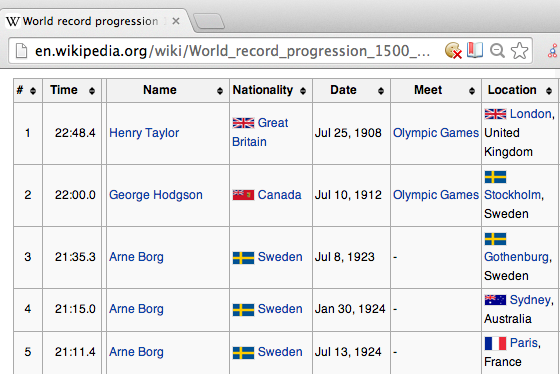
\includegraphics[width=6.5cm]{images/wikipedia_table.png}

\scalebox{.5}{\url{http://en.wikipedia.org/wiki/World_record_progression_1500_metres_freestyle
}}
\end{center}

\end{block}

\end{frame}

%------------------------------------------------

\begin{frame}[fragile]
\frametitle{Reading data in an HTML Table}

To read an HTML table we need to use the function \highcode{readHTMLTable} from the R package \highcode{"XML"}

\begin{knitrout}\tiny
\definecolor{shadecolor}{rgb}{1, 1, 1}\color{fgcolor}\begin{kframe}
\begin{alltt}
\hlcom{# load XML}
\hlkwd{library}\hlstd{(XML)}

\hlcom{# url}
\hlstd{swim_wiki} \hlkwb{=} \hlstr{"http://en.wikipedia.org/wiki/World_record_progression_1500_metres_freestyle"}
\end{alltt}
\end{kframe}
\end{knitrout}

\vspace{3mm}
Since we want the first table, we specify the parameter \highcode{which = 1} 
\begin{knitrout}\tiny
\definecolor{shadecolor}{rgb}{1, 1, 1}\color{fgcolor}\begin{kframe}
\begin{alltt}
\hlcom{# reading HTML table}
\hlstd{swim1500} \hlkwb{=} \hlkwd{readHTMLTable}\hlstd{(swim_wiki,} \hlkwc{which} \hlstd{=} \hlnum{1}\hlstd{,} \hlkwc{stringsAsFactors} \hlstd{=} \hlnum{FALSE}\hlstd{)}
\end{alltt}
\end{kframe}
\end{knitrout}

Note that we can pass \code{data.frame()} parameters, in this case \highcode{stringsAsFactors = FALSE}
\end{frame}

%------------------------------------------------

\begin{frame}[fragile]
\frametitle{Reading data in an HTML Table}

\begin{knitrout}\tiny
\definecolor{shadecolor}{rgb}{1, 1, 1}\color{fgcolor}\begin{kframe}
\begin{alltt}
\hlkwd{head}\hlstd{(swim1500)}
\end{alltt}
\begin{verbatim}
##   #    Time                             Name   Nationality
## 1 1 22:48.4      Taylor , Henry Henry Taylor Great Britain
## 2 2 22:00.0  Hodgson , George George Hodgson        Canada
## 3 3 21:35.3            Borg , Arne Arne Borg        Sweden
## 4 4 21:15.0            Borg , Arne Arne Borg        Sweden
## 5 5 21:11.4            Borg , Arne Arne Borg        Sweden
## 6 6 20:06.6      Charlton , Boy Boy Charlton     Australia
##                           Date          Meet
## 1 01908-07-25-0000Jul 25, 1908 Olympic Games
## 2 01912-07-10-0000Jul 10, 1912 Olympic Games
## 3  01923-07-08-0000Jul 8, 1923             -
## 4 01924-01-30-0000Jan 30, 1924             -
## 5 01924-07-13-0000Jul 13, 1924             -
## 6 01924-07-15-0000Jul 15, 1924 Olympic Games
##                                           Location Ref
## 1 United Kingdom, London !  London, United Kingdom    
## 2           Sweden, Stockholm !  Stockholm, Sweden    
## 3         Sweden, Gothenburg !  Gothenburg, Sweden    
## 4           Australia, Sydney !  Sydney, Australia    
## 5                   France, Paris !  Paris, France    
## 6                   France, Paris !  Paris, France
\end{verbatim}
\end{kframe}
\end{knitrout}

\end{frame}

%------------------------------------------------

\begin{frame}[fragile]
\frametitle{R script and RData}

\begin{block}{R script and RData}
Last but not least, we can also import data inside an R script and in an \highcode{.RData} file. In this case the data files come from John Maindonald's website 
 \begin{itemize}
  \item The table is in the form of an R script \\
{\scriptsize 
\url{http://maths-people.anu.edu.au/~johnm/r/misc-data/travelbooks.R}}
  \item The other type of data is in reality a bunch of data sets in the form of an \code{.RDtat} file \\
{\scriptsize 
\url{http://maths-people.anu.edu.au/~johnm/r/dsets/usingR.RData}}
 \end{itemize}
\end{block}

\end{frame}

%------------------------------------------------

\begin{frame}
\frametitle{travelbooks Data}

Travelbooks Data \low{(by John Maindolnald)}
\begin{center}
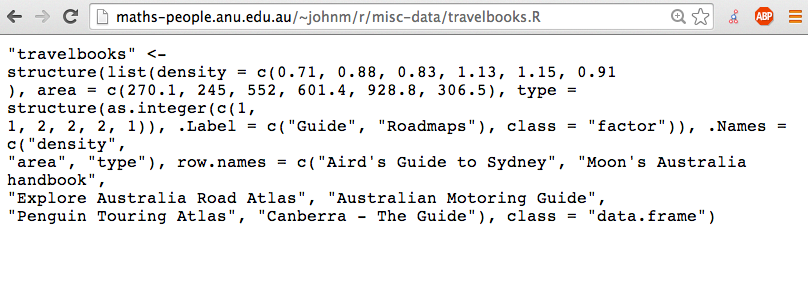
\includegraphics[width=8cm]{images/travelbooks_data.png}
\end{center}

\end{frame}

%------------------------------------------------

\begin{frame}[fragile]
\frametitle{Reading R script with source()}

To read the script we simply need to use the function \highcode{source()}
\begin{knitrout}\tiny
\definecolor{shadecolor}{rgb}{1, 1, 1}\color{fgcolor}\begin{kframe}
\begin{alltt}
\hlcom{# url}
\hlstd{travelbooks} \hlkwb{=} \hlstr{"http://maths-people.anu.edu.au/~johnm/r/misc-data/travelbooks.R"}

\hlcom{# sourcing file}
\hlkwd{source}\hlstd{(travelbooks)}
\end{alltt}
\end{kframe}
\end{knitrout}

\begin{knitrout}\tiny
\definecolor{shadecolor}{rgb}{1, 1, 1}\color{fgcolor}\begin{kframe}
\begin{alltt}
\hlstd{travelbooks}
\end{alltt}
\begin{verbatim}
##                              density  area     type
## Aird's Guide to Sydney          0.71 270.1    Guide
## Moon's Australia handbook       0.88 245.0    Guide
## Explore Australia Road Atlas    0.83 552.0 Roadmaps
## Australian Motoring Guide       1.13 601.4 Roadmaps
## Penguin Touring Atlas           1.15 928.8 Roadmaps
## Canberra - The Guide            0.91 306.5    Guide
\end{verbatim}
\end{kframe}
\end{knitrout}

\end{frame}

%------------------------------------------------

\begin{frame}
\frametitle{RData}

\code{.RData} file \code{usingR.RData} contains several data frames
\begin{center}
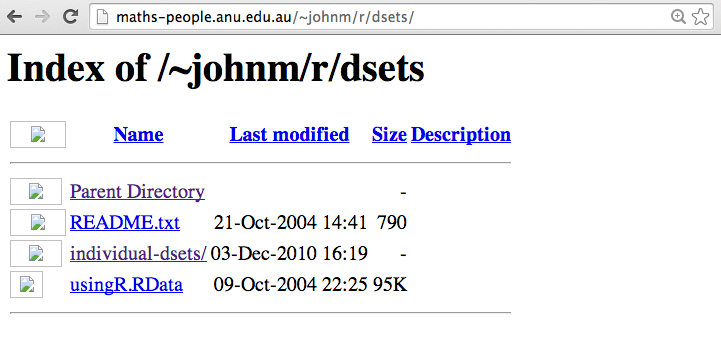
\includegraphics[width=8cm]{images/dsets_data.png}
\end{center}

\end{frame}

%------------------------------------------------

\begin{frame}[fragile]
\frametitle{Reading RData data sets}

For those data sets that are inside an \code{.RData} file, we need to use the function \highcode{load()} and pass the file with \highcode{url()}

\begin{knitrout}\tiny
\definecolor{shadecolor}{rgb}{1, 1, 1}\color{fgcolor}\begin{kframe}
\begin{alltt}
\hlcom{# let's remove all objects in session}
\hlkwd{rm}\hlstd{(}\hlkwc{list}  \hlstd{=} \hlkwd{ls}\hlstd{())}

\hlcom{# url with .RData}
\hlkwd{load}\hlstd{(}\hlkwd{url}\hlstd{(}\hlstr{"http://maths-people.anu.edu.au/~johnm/r/dsets/usingR.RData"}\hlstd{))}
\end{alltt}
\end{kframe}
\end{knitrout}

\begin{knitrout}\tiny
\definecolor{shadecolor}{rgb}{1, 1, 1}\color{fgcolor}\begin{kframe}
\begin{alltt}
\hlcom{# list of read data sets }
\hlkwd{ls}\hlstd{()}
\end{alltt}
\begin{verbatim}
##  [1] "ais"             "alpha_csv"       "alpha_data"      "alpha_xls"      
##  [5] "anesthetic"      "austpop"         "cars2004"        "Cars93.summary" 
##  [9] "dewpoint"        "dolphins"        "elasticband"     "florida"        
## [13] "hills"           "huron"           "i"               "iris_data"      
## [17] "islandcities"    "kiwishade"       "leafshape"       "milk"           
## [21] "moby_dick"       "moby_dick_chap1" "moby_text"       "moths"          
## [25] "mycars"          "myiris"          "myRData"         "myswim"         
## [29] "mytaxon"         "oddbooks"        "one_line"        "orings"         
## [33] "possum"          "primates"        "r_home"          "rainforest"     
## [37] "seedrates"       "skip"            "skulls"          "sw"             
## [41] "swim1500"        "taxon"           "thm"             "tinting"        
## [45] "travelbooks"
\end{verbatim}
\end{kframe}
\end{knitrout}

\end{frame}

%------------------------------------------------

\end{document}
